% !TEX TS-program = pdflatex
% !TEX encoding = UTF-8 Unicode

\documentclass[12pt, a4paper]{article}
\usepackage[utf8]{inputenc}
\usepackage[T1]{fontenc}
\usepackage{helvet}
\usepackage{graphicx}
\usepackage{geometry}
\usepackage{xcolor}
\usepackage[many]{tcolorbox}
\geometry{a4paper, landscape, margin=1.5cm}
\renewcommand{\familydefault}{\sfdefault}
\pagestyle{empty}

% Colors for box styling
\definecolor{boxheaderbg}{HTML}{000000}
\definecolor{boxheaderfg}{HTML}{FFFFFF}
\definecolor{boxcontentbg}{HTML}{F0F0F0}
\definecolor{boxborder}{HTML}{000000}
\definecolor{namebg}{HTML}{D6DEF7}

\begin{document}

% Push the box to the bottom with a 2cm margin
\vspace*{\fill}
\vspace*{-2cm}
\begin{center}
\begin{tcolorbox}[
    width=0.9\textwidth,
    colback=boxcontentbg,
    colframe=boxborder,
    coltitle=boxheaderfg,
    colbacktitle=boxheaderbg,
    fonttitle=\bfseries\sffamily\large,
    title=CHARACTER,
    arc=10pt,
    boxrule=2pt,
    left=8mm,
    right=8mm,
    top=2mm,
    bottom=2mm,
    enhanced,
]
  \begin{minipage}[c]{0.28\textwidth}
    \centering
    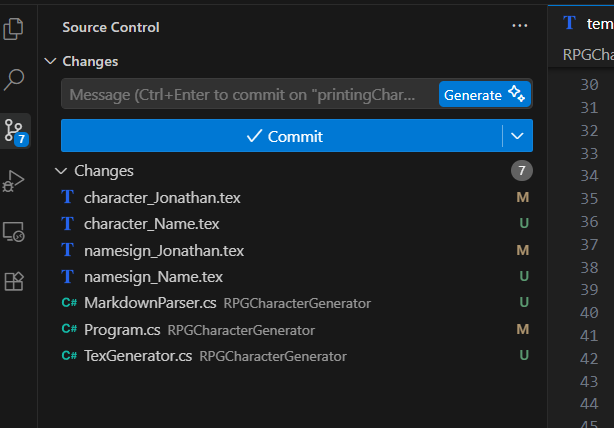
\includegraphics[width=\linewidth, height=6cm, keepaspectratio]{../../images/Nanobana.png}
  \end{minipage}%
  \hfill
  \begin{minipage}[c]{0.68\textwidth}
    \centering
    \vspace{0.5cm}
    \begin{tcolorbox}[colback=namebg, boxrule=0pt, arc=2pt, width=\textwidth, left=0pt, right=0pt, top=2mm, bottom=2mm]
      {\fontsize{38}{44}\selectfont Nanobana}
    \end{tcolorbox}
    \vspace{0.7cm}
    {\large\itshape ""Growth requires patience, but survival requires action.""}
  \end{minipage}
\end{tcolorbox}
\end{center}

\end{document} 
